\documentclass[10pt,a4paper]{article}

\newcommand{\COLORSDIR}{/Users/hoolywear/Desktop/UNIMORE/II ANNO/II SEMESTRE/colors}

\usepackage[italian]{babel}
\usepackage[usenames,dvipsnames]{xcolor}
\usepackage[utf8]{inputenc}
\usepackage[T1]{fontenc}
\usepackage{soul}
\usepackage[a4paper, portrait, margin=2.5cm]{geometry}
\usepackage{array}
\usepackage{tabularx}
\usepackage{multicol}
\usepackage{amsmath}
\usepackage{amsfonts}
\usepackage{amssymb}
\usepackage{algorithmicx}
\usepackage[noend]{algpseudocode}
\usepackage{wrapfig}
\usepackage{graphicx}
\graphicspath{ {./images/} }

\definecolor{emp}{HTML}{f9e9ec}
\definecolor{war}{HTML}{f88dad}
\definecolor{def}{HTML}{fac748}
\definecolor{the}{HTML}{1d2f6f}
\definecolor{obs}{HTML}{8390fa}


\usepackage{listings}

\definecolor{codeblue}{HTML}{074099}
\definecolor{codepurple}{HTML}{850075}
\definecolor{codered}{HTML}{98000f}

\lstdefinestyle{code}{
    backgroundcolor=\color{gray!10},   
    basicstyle=\ttfamily,
    breakatwhitespace=false,         
    breaklines=true,                 
    captionpos=b,                    
    keepspaces=true,                 
    showspaces=false,                
    showstringspaces=false,
    showtabs=false,                  
    tabsize=2,
    mathescape=true %dollar signs act as inline math delimiters
}
\lstdefinestyle{sql}{
    style=code,
    language=SQL,
    commentstyle=\color{codeblue},
    keywordstyle=\color{codepurple},
    stringstyle=\color{codered}
}

\lstset{style=sql}

\usepackage{mdframed}

% styles
\def\Clinewidth{.8pt}
\mdfdefinestyle{titlerule}{%
  frametitlerule=true,roundcorner=5pt,%
  frametitlerulewidth=\Clinewidth,%
  subtitleaboveline=true,subtitlebelowline=true,%
  subtitleabovelinewidth=\Clinewidth,subtitlebelowlinewidth=\Clinewidth,%
subtitlebackgroundcolor=obs,linewidth=1pt}
\mdfdefinestyle{emphasize}{%
  style=titlerule,%
  frametitle=,%
  linecolor=gray!50,linewidth=3pt,backgroundcolor=gray!10,%
  topline=false,bottomline=false,rightline=false}

% verbatim environment
\surroundwithmdframed[backgroundcolor=gray!5,hidealllines=true,%
                      innerleftmargin=1pt,innerrightmargin=1pt%
                      frametitle={}]{verbatim}

% algorithmic environment
\surroundwithmdframed[backgroundcolor=gray!10,hidealllines=true,%
frametitle={}]{algorithmic}

% quote environment
\surroundwithmdframed[style=emphasize]{quote}

% example environment
\newmdenv[frametitle=Esempio,style=titlerule]{example}

% definition environment
\newmdenv[frametitle=Definizione,style=titlerule,%
          linecolor=def]{definition}

% theorem environment
\newmdenv[frametitle=Teorema,style=titlerule,%
          linecolor=the]{theorem}

% emphasize environment
\newmdenv[style=emphasize,%
          linecolor=emp!70!red,backgroundcolor=emp]{emphasize}

% observation environment
\newmdenv[frametitle=Osservazione,%
          backgroundcolor=white,linecolor=obs,%
          frametitlebackgroundcolor=obs]{observation}

% warning environment
\newmdenv[style=emphasize,%
          backgroundcolor=war!10,linecolor=war]{warning}

\author{Iacopo Ruzzier}
\date{Ultimo aggiornamento: \today}


\title{%
Protocolli e Architetture di Rete\\
\large Appunti di teoria}

\begin{document}
\maketitle
\tableofcontents
\newpage
\section{Nozioni introduttive}
\subsection{Compilatori e interpreti}

Il \textbf{compilatore} \`e un componente della toolchain di programmi usati per \textbf{creare eseguibili} a partire da programmi scritti in un qualche \textbf{linguaggio di programmazione}

\begin{minipage}[c]{.65\textwidth}
Altri componenti della toolchain sono
\begin{itemize}
  \item precompilatore
  \item assemblatore
  \item linker (statico e dinamico)
\end{itemize}

Solitamente invoco i componenti mediante un unico \textbf{programma driver}
\end{minipage}
\noindent\begin{minipage}[c]{.35\textwidth}
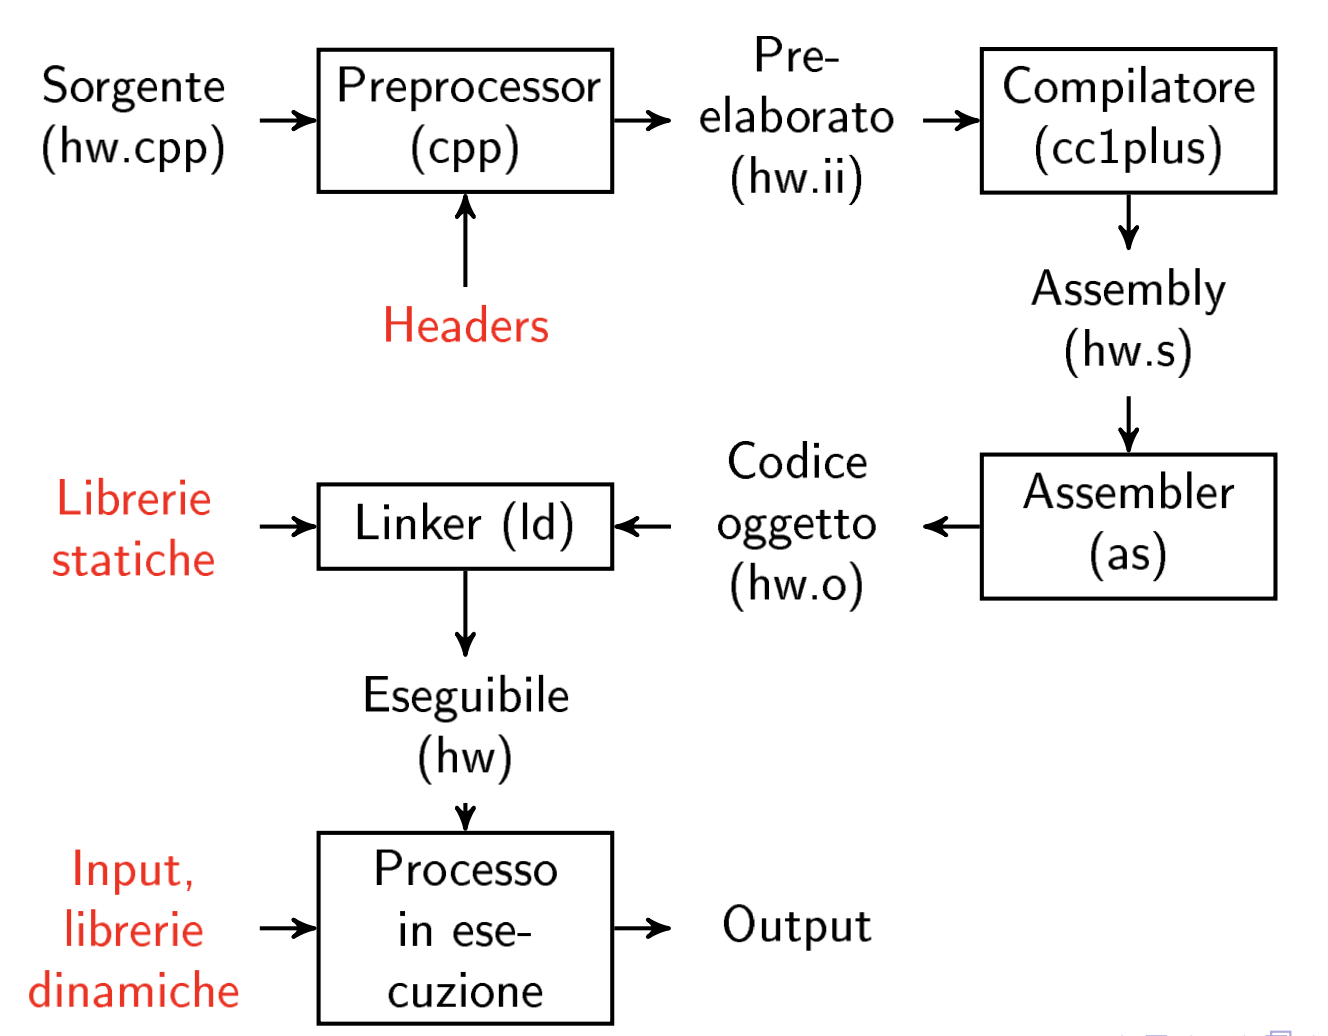
\includegraphics[width=\textwidth]{intro_1.png}
\end{minipage}

\subsubsection{Compilazione con GCC}

La \textbf{Gnu Compiler Collection} o \textbf{GCC} (originariamente acronimo di \textit{GNU C Compiler}) \`e una suite per C/C++, Fortran e Ada. I componenti in relazione a C/C++ ed all'ambiente GNU/Linux sono:

\begin{center}
  \fbox{\lstinline|cpp| $\rightarrow$ \lstinline|cc1/cc1plus| $\rightarrow$ \lstinline|as| $\rightarrow$ \lstinline|ld|}
\end{center}

\noindent con \lstinline|g++| programma driver.

I programmi in uso separato (spesso non in path, a settembre 2024 su distro Debian in \lstinline|/usr/libexec/gcc/x86_64-linux-gnu/XX/|):
\lstinputlisting[language=bash]{listings/lst1/toolchain.sh}
Per determinare i parametri del linker uso \lstinline|g++| con opzione \lstinline|-v| (verbose). Il driver (tra le altre cose) invoca il linker tramite comando \lstinline|collect| (o \lstinline|collect2|), ed elenca i parametri usati:
\lstinputlisting[language=bash]{listings/lst1/toolchain_2.sh}

\subsubsection{Compilatori vs Interpreti}

\textbf{Interpretazione}: impressione di eseguire il programma direttamente in \textbf{linguaggio sorgente}

\begin{figure}[h]
  \centering
  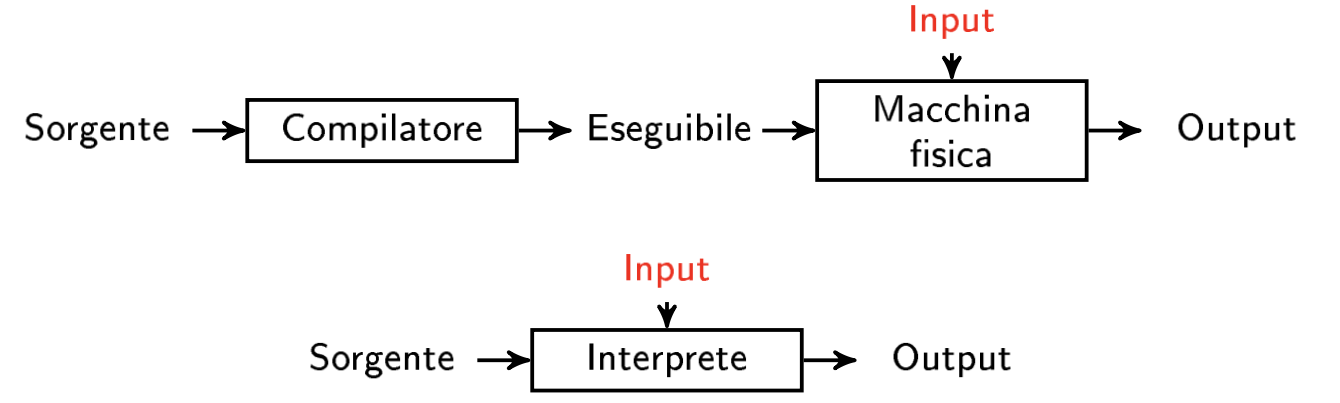
\includegraphics[width=.65\textwidth]{intro_2.png}
\end{figure}


Un interprete \textit{puro} legge il sorgente, lo analizza e lo esegue \textbf{mentre procede} $\rightarrow$ inefficiente (troppo tempo per \textbf{analisi testuale} e \textbf{riconoscimento di espressioni}), usato per pochi linguaggi (es. Lisp originale)

In generale, un'implementazione interpretata include un \textbf{traduttore} (identico al frontend di un compilatore) che fornisce un risultato $\pm$ \textbf{vicino} alla macchina fisica - qui sta la differenza tra i vari interpreti

\paragraph{Modello Perl (Practical Extraction and Report Language)}

\begin{itemize}
  \item la parte iniziale di traduzione produce una rappr. \textbf{ad albero} del programma (AST - Abstract Syntax Tree)
  \item l'interpretazione del programma avviene mediante \textbf{visita post-order} dell'AST (con opportune str.~dati di supporto)\\
  Per maggiore efficienza, vengono prima eseguite svariate \textbf{ottimizzazioni} (es. porzioni da eseguire pi\`u volte vengono tradotte in codice macchina)
\end{itemize}

\paragraph{Modello Java (e Python)}~\\

Tipicamente, il traduttore produce codice \textbf{eseguibile da una VM} $\rightarrow$ \textbf{bytecode}

\begin{emphasize}
    \begin{itemize}
      \item caso Perl: percezione \textbf{analoga all'int. pura} - trad. e int. appaiono come programma unico, l'esecuzione avviene in risposta al singolo comando
      \item caso Java: tr. in bytecode e int. in \textbf{momenti distinti} - ha i moduli distinti \lstinline|javac| e il JRE
    \end{itemize}
    
\end{emphasize}


\subsection{Struttura del compilatore}

(da qui in poi inteso come modulo, non come toolchain completa)

Strutturato in 3 moduli:
\begin{enumerate}
  \item \textbf{front-end}: specializzato nel linguaggio, opera sul sorgente e produce una rappr. intermedia sia \textit{machine} che \textit{language}-independent
  \item \textbf{middle-end}: ottimizza il codice intermedio (focus modulo 2)
  \item \textbf{back-end}: produce il codice per l'architettura target (con specifiche ottimizzazioni)
\end{enumerate}

\paragraph{Passi della compilazione ($4+1+2$)}~\\

\noindent
\begin{minipage}[c]{.55\textwidth}
\begin{itemize}
  \item \textbf{front-end}
    \begin{itemize}
      \item \textbf{analizzatore lessicale}: raggruppa i caratteri in \textbf{token} (parentesi, op, id, ...)
      \item[$\downarrow$] \textbf{analizzatore sintattico}: controlla se i token formano strutture legali e restituisce un \textbf{albero sintattico} (d\`a struttura)
      \item[$\downarrow$] \textbf{analizzatore semantico}: dall'albero s. restituisce un a. \textit{semantico}, ed esegue controlli pi\`u complessi (type check, check sul num. di argomenti passati ad una f. rispetto al num. di parametri formali, ...)
      \item[$\downarrow$] \textbf{generatore di codice intermedio}: dall a. semantico produce la rappr. \textbf{intermedia} (codice corretto e funzionante, \textbf{non ottimizzato}) 
    \end{itemize}
  \item[$\Downarrow$] \textbf{middle-end}
    \begin{itemize}
      \item[$\downarrow$] \textbf{ottimizzatore} sulla rappr. intermedia
    \end{itemize}
  \item[$\Downarrow$] \textbf{back-end}
    \begin{itemize}
      \item \textbf{generatore} + \textbf{ottimizzatore} codice macchina
    \end{itemize}
\end{itemize}
\end{minipage}\hfill
\begin{minipage}[c]{.4\textwidth}
\begin{mdframed}
  \textbf{Tabella dei simboli}: dizionario (tipicam. hash table) che memorizza i simboli \textbf{incontrati man mano} durante l'analisi del sorgente, assieme alle loro caratteristiche (posizione, tipo, ...)
\end{mdframed}
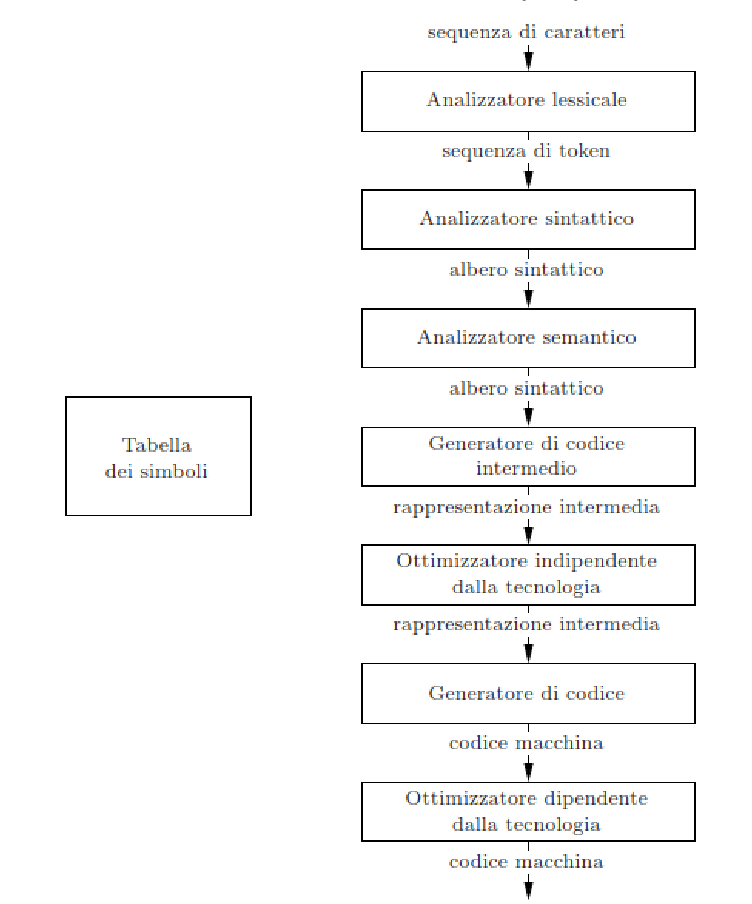
\includegraphics[width=.9\textwidth]{intro_3.png}
\end{minipage}\\




\begin{example}[frametitle={Esempio: fasi applicate ad un'istruzione}]
  \noindent\begin{minipage}[c]{.4\textwidth}
    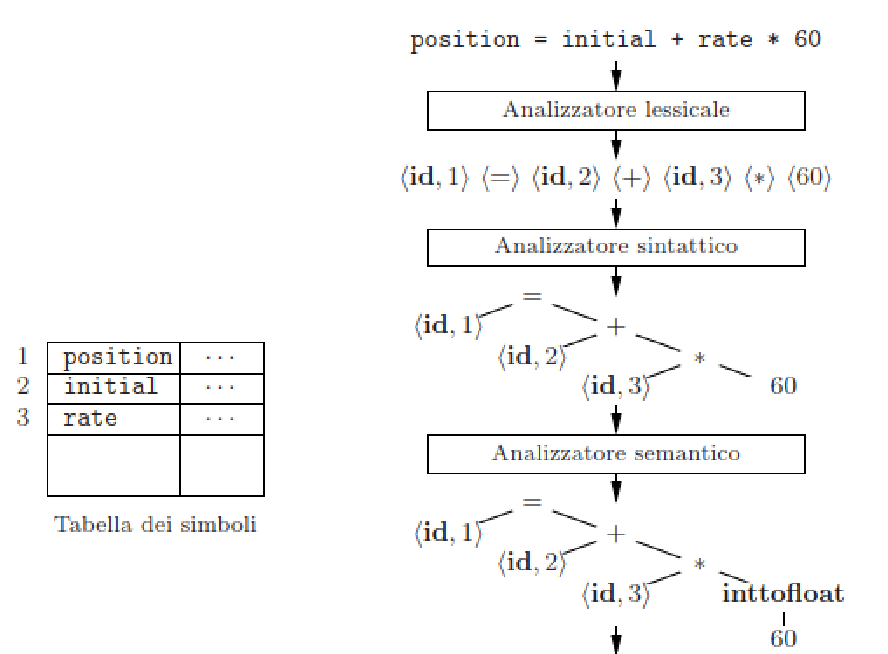
\includegraphics[width=\textwidth]{intro_4.png}
  \end{minipage}\vrule
  \begin{minipage}[c]{.2\textwidth}
    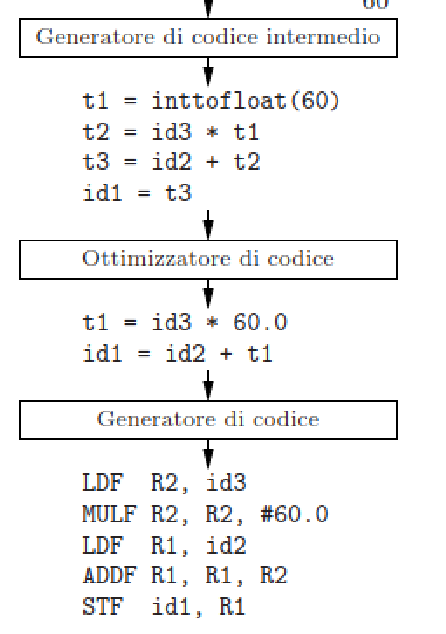
\includegraphics[width=\textwidth]{intro_5.png}
  \end{minipage}
  \begin{minipage}[b]{.4\textwidth}
  \begin{emphasize}
    a passaggio 4, avviene una visita in post-order con spreco di registri intermedi, in cambio per\`o di codice corretto
  \end{emphasize}
  \end{minipage}
  
\end{example}

\subsubsection{Schema riassuntivo (moduli frontend)}

\noindent\begin{minipage}[c]{.6\textwidth}
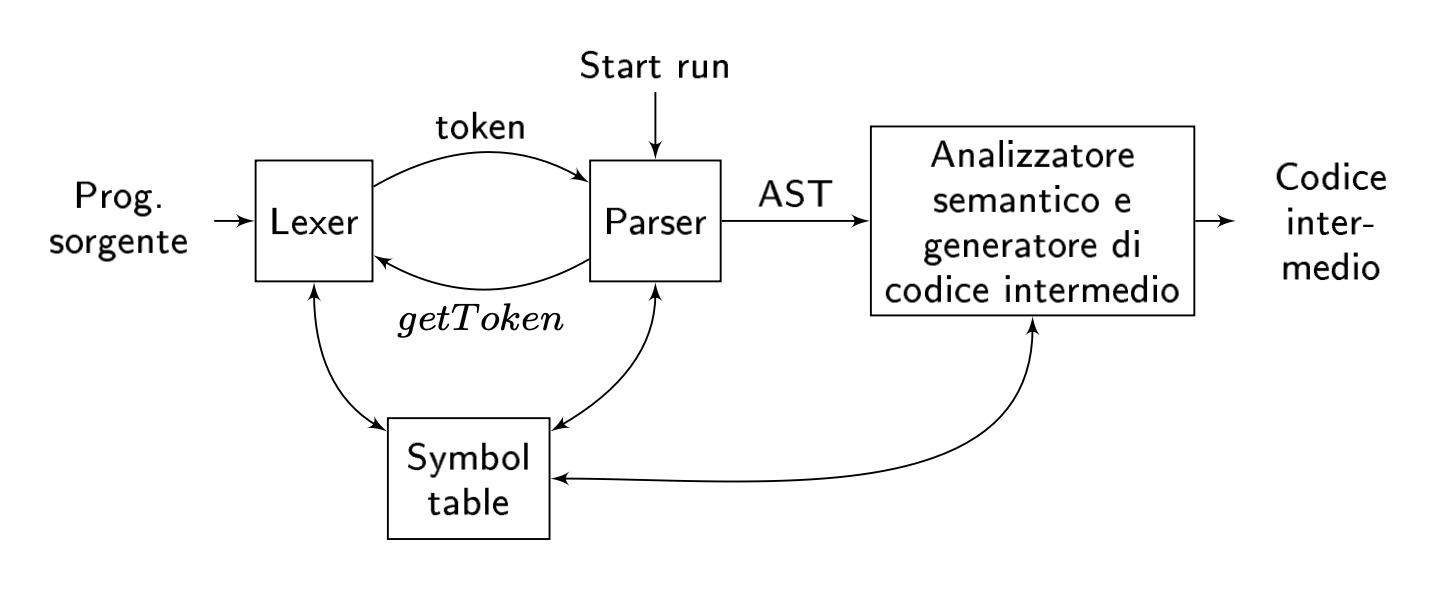
\includegraphics[width=\textwidth]{intro_6.png}
\end{minipage}
\begin{minipage}[c]{.4\textwidth}
  \begin{emphasize}
    Sia per lexer che parser esistono dei generatori, ma lasciano il compito di scrivere \textbf{le regex per identificare i token} (lexer) e le \textbf{regole di com'\`e fatto il linguaggio} (le \textbf{grammatiche formali}) (parser)
  \end{emphasize}
\end{minipage}

\subsection{Alcune nozioni di base}
(da ricordare)

\begin{itemize}
  \item \textbf{type checking}: + o - \textit{forte}; controllo sugli \textit{operandi}; \textit{statico} o \textit{dinamico}
  \item \textbf{regole di scope}: definiscono la \textit{visibilit\`a} delle variabili
  \item \textbf{ambiente e memoria}:
    \begin{itemize}
      \item \textit{ambiente}: mapping tra nomi e locazioni di memoria (\lstinline|int a| modifica l'a.)
      \item \textit{memoria}: mapping tra locazioni di memoria e valori (\lstinline|a = 1| modifica la m.)
    \end{itemize}
    Nei linguaggi formali la memoria \textbf{non si vede} (mapping diretto nomi-valori senza puntatori)
  \item \textbf{$l$-value e $r$-value}:
    \begin{itemize}
      \item $l$-value: oggetti con posizione di memoria identificabile (es. id)
      \item $r$-value: valori a destra di \lstinline|=|
        \begin{lstlisting}
int x; int *p;
p = &x # legale
&x = p # illegale
l-value = r-value # in generale\end{lstlisting}
    \end{itemize}
  \item \textbf{implementazione} di
    \begin{itemize}
      \item \textbf{stack} (pila - linked list)
      \item \textbf{dizionario} (hash map, dict)
      \item \textbf{albero binario} (struct con 2 puntatori, array paralleli; info, indice sx, indice dx)
      \item \textbf{albero n-ario} (array paralleli non utilizzabili: struct con puntatori \lstinline|left| e \lstinline|next-sibling|)
    \end{itemize}
    
\end{itemize}

\section{Linguaggi formali}
\section{Linguaggi regolari}
\section{Analizzatore lessicale (lexer)}
\section{Sintassi e grammatiche}

\end{document}
